\documentclass[UKenglish]{ifimaster}  %% ... or USenglish or norsk or nynorsk
\usepackage[latin1]{inputenc}        %% ... or utf8 or applemac
\usepackage[T1]{fontenc,url}
\urlstyle{sf}
\usepackage{babel,textcomp,csquotes,ifimasterforside,varioref,graphicx}
\usepackage[section]{placeins}
\usepackage{amsmath}


\usepackage{listings}
\usepackage{color}

\definecolor{mygreen}{rgb}{0,0.6,0}
\definecolor{mygray}{rgb}{0.5,0.5,0.5}
\definecolor{mymauve}{rgb}{0.58,0,0.82}

\lstset{ %
  backgroundcolor=\color{white},   % choose the background color; you must add \usepackage{color} or \usepackage{xcolor}
  basicstyle=\footnotesize,        % the size of the fonts that are used for the code
  breakatwhitespace=false,         % sets if automatic breaks should only happen at whitespace
  breaklines=true,                 % sets automatic line breaking
  captionpos=b,                    % sets the caption-position to bottom
  commentstyle=\color{mygreen},    % comment style
  deletekeywords={...},            % if you want to delete keywords from the given language
  escapeinside={\%*}{*)},          % if you want to add LaTeX within your code
  extendedchars=true,              % lets you use non-ASCII characters; for 8-bits encodings only, does not work with UTF-8
  frame=single,                    % adds a frame around the code
  keepspaces=true,                 % keeps spaces in text, useful for keeping indentation of code (possibly needs columns=flexible)
  keywordstyle=\color{blue},       % keyword style
  language=Octave,                 % the language of the code
  morekeywords={*,...},            % if you want to add more keywords to the set
  numbers=left,                    % where to put the line-numbers; possible values are (none, left, right)
  numbersep=5pt,                   % how far the line-numbers are from the code
  rulecolor=\color{blue},         % if not set, the frame-color may be changed on line-breaks within not-black text (e.g. comments (green here))
  showspaces=false,                % show spaces everywhere adding particular underscores; it overrides 'showstringspaces'
  showstringspaces=false,          % underline spaces within strings only
  showtabs=false,                  % show tabs within strings adding particular underscores
  stepnumber=0,                    % the step between two line-numbers. If it's 1, each line will be numbered
  stringstyle=\color{mymauve},     % string literal style
  tabsize=2,                       % sets default tabsize to 2 spaces
  title=\lstname                   % show the filename of files included with \lstinputlisting; also try caption instead of title
}



\setlength{\parskip}{\baselineskip}%
\setlength{\parindent}{0pt}%


\title{Do Work in Progress (WIP) - Limit in Agile Software Development Matter?}        %% ... or whatever
\author{Truls Skeie}                      %% ... or whoever 
\usepackage[
    backend=biber,
    style=authoryear-icomp,
    sortlocale=de_DE,
    natbib=true,
    url=false, 
    doi=true,
    eprint=false
]{biblatex}
% !BIB TS-program = biber

\addbibresource{lib.bib}

\begin{document}
\ififorside{}
\frontmatter{}
\maketitle{}

\chapter*{Abstract}                   %% ... or Sammendrag or Samandrag

\tableofcontents{}
\listoffigures{}
\listoftables{}

\chapter*{Preface}                    %% ... or Forord

\mainmatter{}
\part{Introduction}                   %% ... or Innledning or Innleiing


\chapter{Background}                  %% ... or Bakgrunn
In the field of WIP and if WIP matters in software development, lacks proper research, but Giulio Concas and Hongyu Zhang has done research on the difference between limit WIP and unlimited WIP  \parencite{SMR:SMR1599}.

Work in progress is a tool that helps teams limits their tasks by specifying how many tasks a developer can be assigned to at once. WIP helps team to reduce overhead, decrease leadtime and increase throughput %%finne reff

How to find the best WIP in a given interval and context also lacks proper research, but in manufacture business some research has been done. Taho Yanga, Hsin-Pin Fub, Kuang-Yi Yanga stated that WIP could be defined as; WIP = cycle time * throughput rate in manufacture business \parencite{Yang}.

\section{Kanban}
''We can define Kanban software process as a WIP limited pull system visualized by the Kanban board''  \parencite{DavidAnderson}.

Kanban system focus on;
\begin{itemize}
\item Continuous flow of work
\item	No fixed iterations or sprints
\item Work is delivered when it?s done
\item Teams only work on few tasks at the time specified by the limit WIP
\item Make constant flow of released tasks
\end{itemize}
\parencite{DavidAnderson}.

Toyota production system was introduced Kanban during late 1940s and early 1950s in order to catch up with the American car industry \parencite{ono1988toyota} . In the last ten years software Development Company have started to implement agile methods and Kanban is one of them \parencite{Conboy}.  Kanban splits one big problem into many small pieces of problems.

When the small pieces are in order, the problems are put up on the Kanban-board to visualize the problems and see potential bottlenecks. When people started to understand Kanban, they easily discovered where the bottlenecks where, and started to help where the bottlenecks where \parencite{Shinkle}.

One of the most important people in Kanban software development, David Anderson  also referred to as ''father of Kanban in the software development industry''  \parencite{InfoQ:2013:May:Online}, author of Kanban: Successful Evolutionary Change for Your Technology Business once stated ''If you think that there was Capability Maturity Model Integration, there was Rational Unified Process, there was Extreme Programming and there was Scrum, Kanban is the next thing in that succession.''   \parencite{InfoQ} 

More and more software projects adapt to Kanban, and this is one of the reasons why this thesis will focuses on Kanban and WIP.
Kanban is one of the agile method in the wind these days, and is used with Lean Software development which is one of the fastest growing approaches in software development \parencite{DavidAnderson}

One of the main difference between Scrum and Kanban is estimation, in simulation of software maintenance process, with and without a work-in-process limit \parencite{SMR:SMR1599} estimation was defined to be the main source of waste. In their research, they find out, if they let the developers work with small tasks at time and not be interrupted, they will be more effective. The developers in this case was interrupted when they was assigned to estimate tasks. The research groups decided to implement Lean-Kanban, which includes minimizing waste, which meant estimation for this case. After implementing Lean-Kanban the teams increased the ability to perform work, lower the lead time and meet the production dates.

\section {Scrum}
Scrum has three main roles, the Product Owner, the Scrum Master and the members of the development team. The Product owner in collaboration with the Scrum Master decides which work to be prioritized in the backlog. The Scrum Master acts like a team leader and helps the team and organization to take best advantages of Scrum. The development team works on tasks specific for the iteration there in  \parencite{Scrum}.

Iteration is a time-boxed interval over a given time, usually from one to four weeks. Before each sprint, a sprint planning meeting is conducted, with all the team members attending  \parencite{Scrum}.

In each sprint a minimal backlog is created so the developer knows which tasks to work on. The Product Owner and the team members discuss and decide which tasks from the backlog to be added to the minimal backlog  \parencite{Scrum}.

After the minimal backlog is full, the Product Owner and the team members discuss each task from in order to get a better understanding and a shared understanding of what is required in order to complete the task  \parencite{Scrum}.

Scrum requires that a new feature is ready for release after a sprint. The feature should be a visible part of the product in order to get feedback from end-users  \parencite{Scrum}

\section {Lean-Kanban}
The Lean approach was introduced between 1948 and 1975 in manufacturing work in Japan. It was designed to find and eliminate waste, so the manufacturing could deliver value to the costumer more efficiently. In 2003 Mary and Tom Poppendieck first introduced Lean thinking to software development, they published ?Principles of Lean Thinking? \parencite{Lean:2003}. An important tool to manage work flow is the concept of pull-systems, which means tasks are put in production only when a costumer asks for it \parencite{Lean:2009}.
In the last years, Kanban has been introduced more and more to software development, and is becoming one of the keys to Lean practice in the field \parencite{DavidAnderson}. 

\section{WIP}
''There's stated when using short-cycle times and Kanban board to limit WIP, the software development team's learning is increased'' \parencite{Joyce}

Work in progress (WIP) is a tool in Kanban to reduce overhead by limit task-switching for each developer and visualize bottlenecks. Each column in a Kanban board usually has a specific WIP as illustrated in figure \ref{kanban_board}.  

WIP can be explained using cars and roads as analogy. All roads have it maximum capacity width number of cars. When this limit is reached, traffic jam occurs and the throughput of cars decreases and lead time increases. The same can be said about software development teams, a software team has a maximum number of tasks they can perform, if the team is pushed over the maximum limit, the throughput of tasks decreases and lead time increases.
 
But in order to get the best throughput and lead time, a software team needs to experiment with WIP. 
When first implementing Kanban, Shinkle explains that the users don't care about the WIP, but rather the visibility of Kanban. When the user gets more experience with Kanban, they start to attempt limit WIP \parencite{Shinkle}
Shinkle defined novice and more experience kanban-users with a descriptive analogy \parencite{Shinkle}:
''Think about a typical person wanting to bake a cake. They go to the store, purchase a boxed cake mix, and follow the directions as described on the back of the box. They have little to no knowledge about how to alter the recipe nor do they have a desire to do so. Their goal is simply to bake a cake.''
''An advanced beginner understands how to apply some context to the instructions or rules on the back of the box. They can make minor adjustments for things like altitude, pan size, oven conditions, etc. They are still following the basic recipe, but can make minor adjustments likely based on previous experiences.''
In the paper Applying the Dreyfus Model of Skill Acquisition to the Adoption of Kanban Systems at Software Engineering (SEP) \parencite{Shinkle}, Shinkle interview some developers and one developer said:
?WIP limits seem to be the worst understood part of the Kanban system. When used properly, it exposes bottlenecks and reduces lead time for individual work items. Used improperly, it can starve developers for work or result in too many people working on the same work items.'' \parencite{Shinkle}
 
Setting a limit on WIP has a number of benefits according to Hopp, Spearman and Suri. They stated that it reduces flow times, reduces variation and improves quality. However Srinivasan, Ebbing and Swearing said that setting the WIP is not easy. They suggest that WIP are just set, and then observe throughput, and adjust after that \parencite{Mandyam}.
Several people have their opinion on how to best measure the WIP, but most of them agree upon that's there is no clear rule of how to measure WIP in software development. Lukasz proposes to use The Effectiveness as an indicator measured at the end of each cycle. The effectiveness is a formula that takes the number of bugs found (ai) and the number of bugs found by external people (e.g. lawyers, accountants, coaches, consultants, translators, internal and external service providers ,etc.)(ei), and minus ai and ei, then divide the result by ai and multiply it by 100\%  as shown in \ref{WIPEQ} \parencite{Sienkiewicz}

\begin{equation} \label{WIPEQ}
Ei=\frac{ai-ei}{ai}*100\%
\end{equation}

On the other hand, Kanban says you should limit WIP. So what should the limit be? - Kanban; Don't know, experiment \parencite{Kniberg}.

Lean Software Management suggest that WIP should be minimized, to keep high quality \parencite{Ikonen} and to create continuous flow and bring problems to the surface \parencite{Joyce}. In Lean Software Management: BBC Worldwide Case Study when the team realized the where bottlenecks and to high WIP the team started to determine WIP by their constraints. The team quickly realized that they had fewer quality assurance/testing staff and business analysts than software developers. This reflected the bottlenecks, so the team adjusted WIP to how much work they could handle; this gave the team more experience in dealing with WIP \parencite{Joyce}.

In the authors of Lean thinking in software development: Impacts of kanban on projects suggest that task should be prioritized from high to low, in order to keep the best WIP. Lean thinking in software development: Impacts of Kanban on projects stated in the conclusion that high WIP will keep people task switching and not be able to fully concentrate on each work in progress \parencite{Ikonen}.
As notice, there?s no clear rule on how to deal with WIP and how to determine WIP, although WIP is a crucial tool in order to Kanban sufficient

\section {Kanban Board}
''The Kanban board makes it clear to all the team members the exact status of progress, blockages, bottlenecks and they also signal possible future issues to prepare for''\parencite{Joyce}.

The Kanban board is one of the most important tools in Kanban. It?s used to minimize WIP, increase the information flow, with visualization  and spot bottlenecks \parencite{SMR:SMR1599}.
The Kanban board uses named columns to illustrate where each item is in the workflow.  Every column has a WIP, to specify how many works in progress there are allowed in the column \parencite{Joyce}.
A Kanban board is illustrated in figure \ref{kanban_board}, where each column has a name respectively Backlog, In progress and done.
\begin{figure}[ht!]
\centering
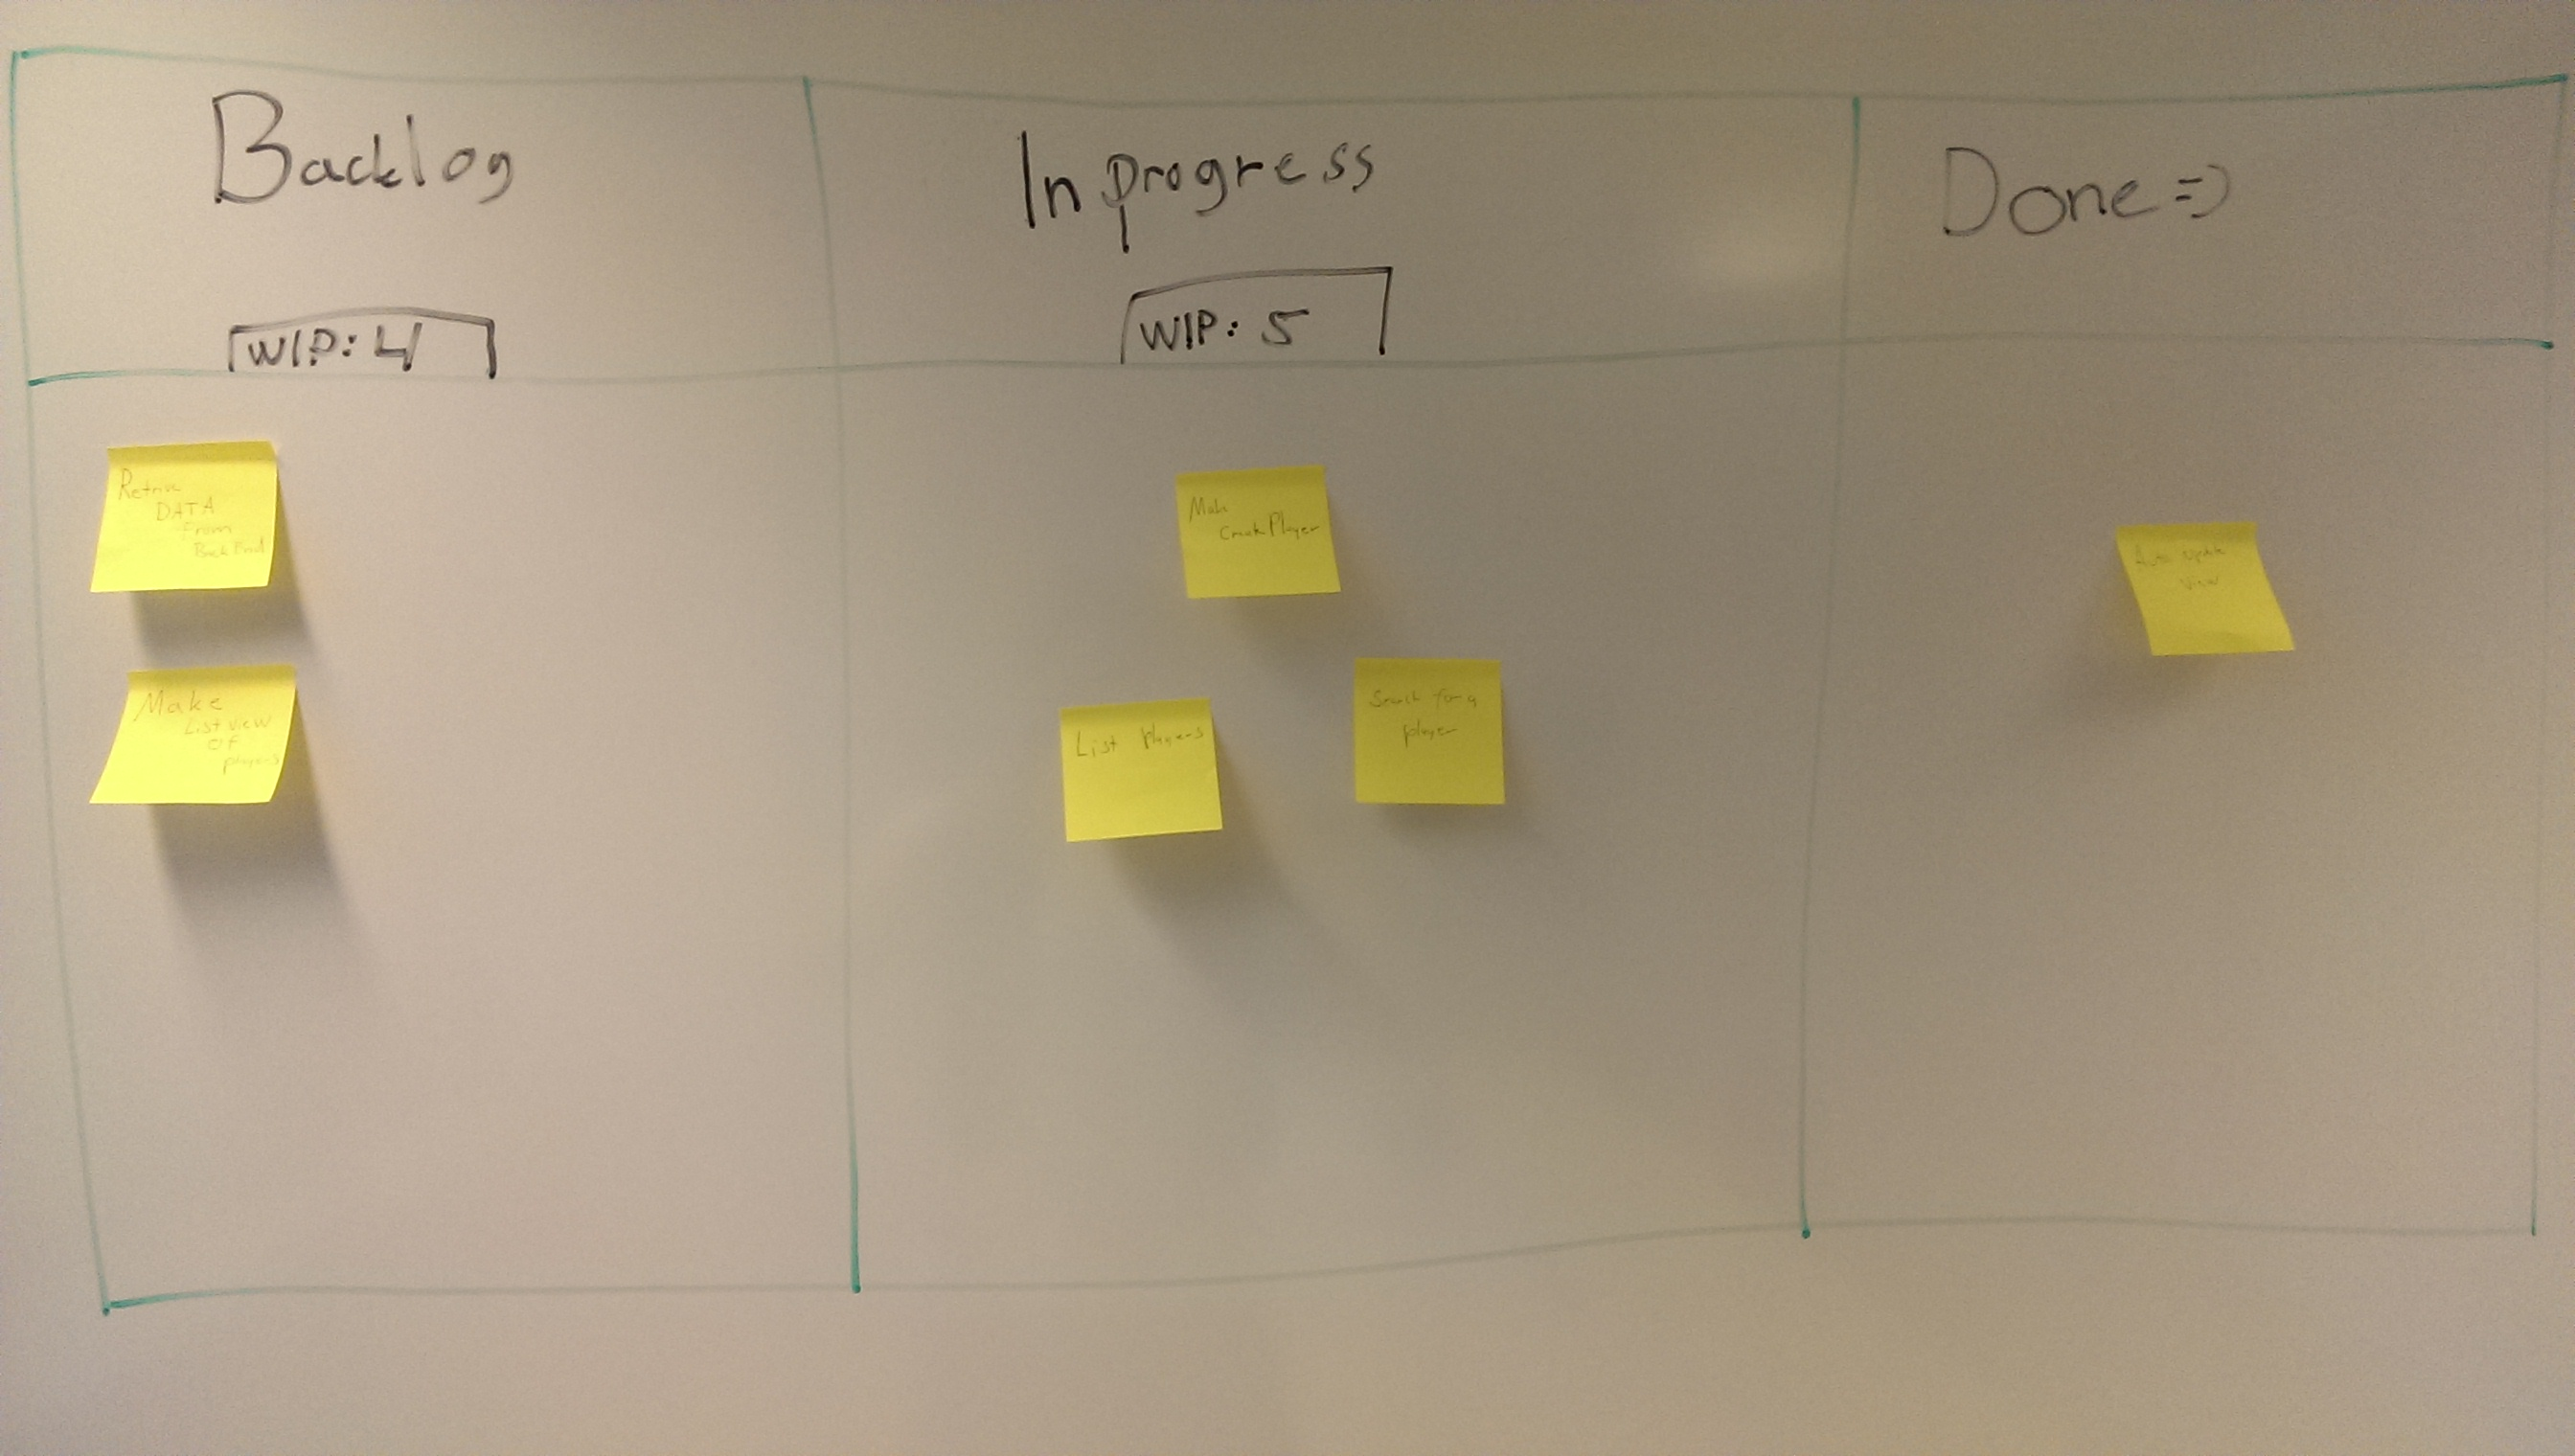
\includegraphics[width=90mm]{Picture/kanban_board.jpg}
\caption{Example of a Kanban board}
\label{kanban_board}
\end{figure}

\section {Lead time}
''Lead time is the total elapsed time from when a customer requests software to when the finished software is released to the custome'' \parencite{Joyce}.
The citation by Joyce above is the close to definition of what lead time is. This definition could be useful for consultancy companies, but for SI, who is a big in-house development company with few releases each year this definition is unsuitable. Quantifying the effect of Using Kanban versus Scrum stated to definition of why the definition is unsuitable: 

''First, the amount of time a work item remains in the backlog queue before it's put on the board is a function of priority, not whether the company uses Scrum, Kanban, or other development methods. Furthermore, companies that develop and sell products to many customers might propose new features themselves and put them on the backlog before any customers request them. Second, given a policy of two or three releases a year, the result of a work item isn't delivered to the customer immediately after it's finished'' .
\parencite{Dag}

As long as SI has defined what Lead time is in their case, lead time could be used as an essential ingredient when you look for the optimal WIP for their project, because with lead-time, they can control the timer interval for each task. Often in project, lead time is split into pieces, so every task has its own lead-time; this gives the development teams the advantages to experiment with different WIP's in order to see the different lead-times and then measure which WIP that suits this project the best. 

\section{Throughput}
''The average output of a production process (machine, workstation, line plant) per unit time (e.g., parts per hour) is defined as the systems throughput or sometimes throughput rate'' \parencite{Adams}

The concept of throughput in order to measure how productive teams, people or companies is similar in both software development and manufacturing. But, in software development each tasks is abstract, tasks can have different solutions depending on how the team or developer approach and the tasks is usually only done once.

In manufacturing, each task usually has one solution and when the solutions are found the physical item is mass produced.  Adams said "Throughput in plant, line or workstation, is defined as the average quantity of good  parts produced per unit time" \parencite{Adams}, which gives a good example of the relationship between tasks in manufacturing and software development. In manufacturing the part either fits its purpose (good) or not (defective), in software development a tasks can fit a purpose, but the purpose may be wrong. As long as the software development task is bug free, it's delivered as non-defective but it may not fit the defined purpose by the end users. 

Throughput is measured in number of finished delivered tasks per day, week, month, quarter or year. In order to make throughput measurement successful, each tasks has to require almost the same amount of work.  

For instance; team x had a throughput of ten after the first quarter, twenty after the second, fifteen after the third and twelve after the last quarter and they used Scrum the first two quarters and Kanban the last two as illustrated in table \ref{tt}
It will look like team x benefits most from Scrum. But if the task during the Kanban time was twice the size of Scrum, the Kanban approach would fit them better than Scrum. In order to find that out, the team x needs to standardize how much work each tasks should require.

\begin{table}[ht]
\begin{center}
    \begin{tabular}{| l | l | l | l |}
    \hline
    Quarter & Throughput &  Framework\\ \hline
    1 & 10 & Scrum\\ \hline
    2 & 20 & Scrum \\ \hline
    3 & 15 & Kanban\\ \hline
    4 & 12 & Kanban\\ \hline
    \end{tabular}
\caption{Throughput}
\label{tt} %% throughput table
\end{center}
\end{table}

\section{Chrun}
%%fylle inn?
\section {Limit WIP vs. Unlimited WIP}
There's been done some research on how the throughput, leadtime and how developers experience WIP limit and unlimited WIP

Simulation of software maintenance process, with and without a work-in-process limit has done research on limit WIP vs. unlimited WIP, one of the result from this paper was at the end of a simulation, the average of closed issued was 4145 when the WIP was limited and 3853 when the limit was not limited (about 7\% less). The paper concludes their finds like; developers are more focused on fixing few issues, because the number of issues they can work on is limited.  Because the limit of WIP, the developers are more likely to continue on the issue from the day before, rather than starting on another issue, this reduce overhead. When developers start on a new issue, they need to use time to familiarize themselves with the code and the issue. That could create unnecessary overhead if some developer already has done it, but that developer is now working on a another issue \parencite{SMR:SMR1599}.

\section{Software Innovation(SI)}
Software Innovation is a Scandinavian software company. SI develops and delivers market-leading Enterprise Content Management applications that helps organizations improve and increase efficiency in document management, case handling and technical document control.

Software Innovation has approximately 300 employees, and has offices in Oslo, Copenhagen and Stockholm and a development center in Bangalore \parencite{SI}.


\part{The project}                    %% ... or ??
\chapter{Research Questions}
In this thesis the overall research question in this thesis is to study the effects of WIP limits in particular for SI. Some of the goals are:
\begin{itemize} 
\item See if the exist an optimal WIP-limit for a given context.
\item How to best find the optimal WIP-limit
\item Which various parameters taking in to account in order to optimize WIP. 
\end{itemize}
\chapter{Research Methods}
%%Skrive om weekends
In this section information about how my program will measure WIP, Items in backlog and throughput per date, per month, per quarter and per year will be explained. First off, there will be describe how the program do the measure in words, then the algorithm will be explained using algorithm in Pseudocode \parencite{jd}

The set from SI only contains dates when tasks was created, added to backlog, pulled from backlog or finished.  In order to measure average per month, quarter and year the program needs to know WIP and items in backlog for each day. In order to do so, the program will generate the remaining days.

Table \ref {dataset} show an excerpt from the dataset, as the reader may notice, the date 2008-10-09 is not in the set, so in this case, the program has to create 2008-10-09 and add it to the set

\begin{table}[ht]
\begin{center}
    \begin{tabular}{| l | l | l | l |}
    \hline
    Created Date\\ \hline
    2008-10-07\\ \hline
    2008-10-07 \\ \hline
    2008-10-07 \\ \hline
    2008-10-08\\ \hline
    2008-10-08\\ \hline
   2008-10-10\\ \hline
    \end{tabular}
\caption{Excerpt from the dataset}
\label{dataset} %% throughput table
\end{center}
\end{table}

The Date standard is specified as yyyy-mm-dd. \\
When I write iterate it means looping through the data with a for each-loop. \\
Quarter of a year is defined as January, February and March (Q1); April, May and June (Q2); July, August and September.\\ (Q3); and October, November and December (Q4) according to Investopedia \parencite{Quarter}

\section{Analyzed Data}
In this thesis the plan is to measure the data in one big step, where I measure all the teams and data in some given interval. I would also measure the data in small steps, when SI used Scrum, when SI was in the transforming phase and when they had changed to Kanban. Also I will measure WIP values for a given day, date, week, month, quarter and year. This will give me data to compare between teams in a specific interval.

I will reuse some data from the paper from Quantifying the Effect of Using Kanban vs. Scrum: A Case Study \parencite{Dag} Mainly I will look at churn and lead-time measured in the paper and compare them with WIP and throughput between teams. Hopefully the data measured will give me some sense of what WIP limit does for SI and which factors helping determine if WIP-limit matters in agile software development

Hopefully I would gather or get some other underlying data, so I will be able to compare my work, on the set from SI to the other data.

\section{Information about the dataset}
The set from SI contains almost thirty columns of different data. I will not examine every column in my thesis, but the columns I will use will be given a brief introduction to here.
\newpage
\subsection{The columns}
\begin{table}[ht]
\begin{center}
    \begin{tabular}{| l | p{5cm} |}
    \hline
     Column & Description\\ \hline
     Created Date & When a task is put in backlog \\ \hline
     Date From & When a given task is taken from the backlog\\ \hline
     Date to & When a task is done. Done is defined by SI to be ready for release. \\ \hline
    Lead Time & The amount of time elapsed from the date the task was created until the tasks has finished  \\ \hline
   Process Type &States the process used by the team which contains Kanban or Scrum \\
    \hline
    Team &States the team who has been working on the task.\\ \hline
    \end{tabular}
\caption{Information about the columns from the SI dataset}
\label{IC} %% information columns
\end{center}
\end{table}

\subsection {Algorithms for calculating WIP, backlog and throughput}
\begin{table}[ht]
\begin{center}
    \begin{tabular}{| l | l | p{5cm} |}
    \hline
    Variable &	Description	 & Columns from SI\\ \hline 
    Wip-Limit per day & \parbox[t]{5cm}{The number of items in progress on the given day} & Date From and Date To. \\ \hline
    Throughput	& Number of tasks finished on a given day & Date To \\ \hline
    Backlog & Number of items in backlog on a given day & Created Date and Date From\\ \hline
 Hashmap &\parbox[t]{7cm}{Hash table algorithm works by associating keys and their values in one-to-one mapping and storing them in a hashmap \parencite{Hashmap}} & \\ \hline
\end{tabular}
\caption{Description of variable and which columns from the SI set that is used to measure the variable}
\label{IC} %% information colum    
\end{center}
\end{table}

\begin{table}[ht]
\begin{center}
    \begin{tabular}{| l | p{5cm} |}
    \hline
     Key - Date  & Value - Integer\\ \hline
     2008-10-07 & 2   \\ \hline
     2008-10-08 & 0   \\ \hline
     2008-10-09 & 0   \\ \hline
     2008-10-10 & 2   \\ \hline
     2008-10-11 & 3   \\ \hline
     2008-10-12 & 0   \\ \hline
     2008-10-13 & 0   \\ \hline
     2008-10-14 & 2   \\ \hline
     2008-10-15 & 0   \\ \hline
     2008-10-16 & 0   \\ \hline
     2008-10-17 & 0   \\ \hline
     2008-10-18 & 0   \\ \hline
     2008-10-19 & 0   \\ \hline
     %%hva er dette til?
    \end{tabular}
\caption{skrive noe spennede}
\label{IC} %% information columns
\end{center}
\end{table}

\subsection {WIP-limit per day}
In order to describe the algorithm of measuring WIP limit per day, I will do it stepwise.  A detailed example on how the algorithm works is listed in the \ref{sec:Example}.

\subsection{Step 1: Gather all dates into a Hashmap}
First step of WIP measurement is adding every date in the date from column into a hashmap. Hashmaps contains key-value pairs, which will be respectively Date and Integer in this algorithm.  The date will contain the 'date from' column and the counter is number of occurrence of the date also known as WIP for that date. 
 \begin{lstlisting}
FOR date IN date_from_column:
WIP = nr_of_date_ occurrence(date)
Hashmap.put(date, WIP)

nr_of_date_ occurrence(Date date) 
FOR d IN date_from_column DO
	IF d EQUAL date DO
		nr_of_date_ occurrence++
RETURN nr_of_date_ occurrence
 \end{lstlisting}
\subsection{Step 2: Gather the remaining days}

\subsection{Step 3 Measure WIP}

\subsection{Example}
\label{sec:Example}



\chapter{Planning the project}        %% ... or ??


\part{Conclusion}                     %% ... or Konklusjon

\chapter{Results}                     %% ... or ??


\backmatter{}
\printbibliography
\end{document}
